\section{TensorFlow API}
\subsection{Sequential API}
\begin{itemize}
    \item Birbirini takip eden sıralı katmanlardan model oluşturmayı sağlar.
    \item Modelin yalnızca 1 giriş ve 1 çıkışı vardır.
\end{itemize}

\subsubsection{Python Kodu}

\begin{lstlisting}[language=Python]
import tensorflow as tf

model = tf.keras.Sequential([
    tf.keras.layers.Dense(128, activation='relu', input_shape=(784,)),
    tf.keras.layers.Dropout(0.2),
    tf.keras.layers.Dense(10, activation='softmax')
])

model.compile(optimizer='adam',
              loss='sparse_categorical_crossentropy',
              metrics=['accuracy'])

model.summary()
\end{lstlisting}

\begin{figure}[ht]
    \centering
    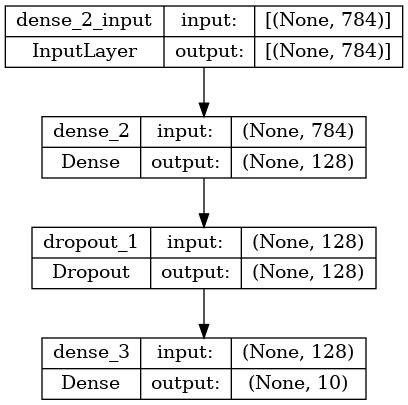
\includegraphics[width=0.6\textwidth]{images/sequential_model.png}
    \caption{Sequential API ile oluşturulan modelin mimarisi.}
    \label{fig:enter-label}
\end{figure}

\newpage

\subsection{Functional API}
\begin{itemize}
    \item Esnek bir yapıdadır. Dallanmış veya birleştirilmiş yapılar gibi karmaşık model yapılarını oluşturmayı sağlar.
    \item Modelin birden fazla giriş ve çıkışı olabilir.
\end{itemize}

\subsubsection{Python Kodu}

\begin{lstlisting}[language=Python]
import tensorflow as tf

inputs = tf.keras.Input(shape=(784,))
x = tf.keras.layers.Dense(128, activation='relu')(inputs)
x = tf.keras.layers.Dropout(0.2)(x)
outputs = tf.keras.layers.Dense(10, activation='softmax')(x)
model = tf.keras.Model(inputs=inputs, outputs=outputs)

model.compile(optimizer='adam',
              loss='sparse_categorical_crossentropy',
              metrics=['accuracy'])

model.summary()
\end{lstlisting}

\begin{figure}[ht]
    \centering
    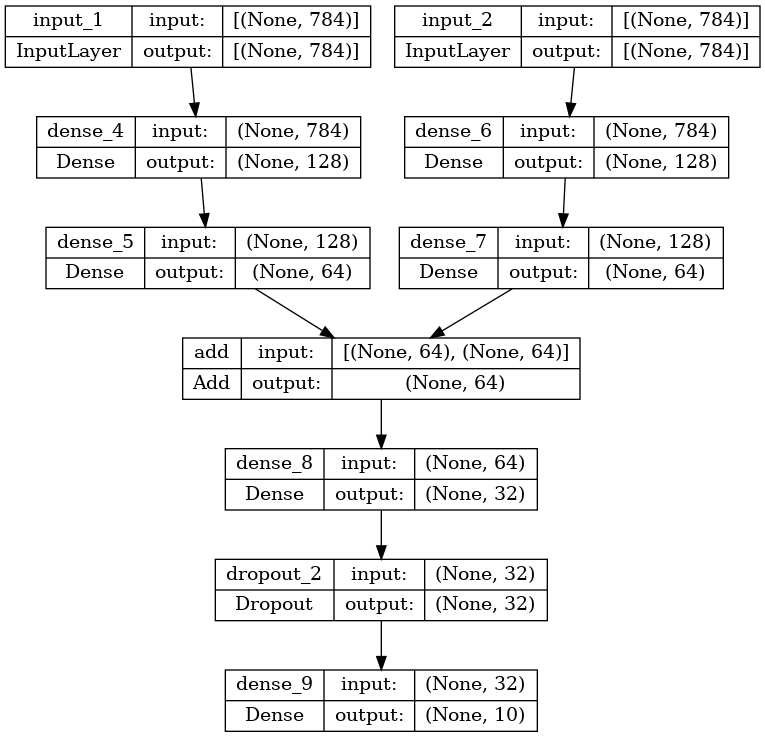
\includegraphics[width=0.6\textwidth]{images/functional_model.png}
    \caption{Functional API ile oluşturulan modelin mimarisi.}
    \label{fig:enter-label}
\end{figure}

\newpage